\documentclass{article}

% 导入宏包
\usepackage{fancyhdr}
\usepackage{ctex}
\usepackage{listings}
\usepackage{graphicx}
\usepackage[a4paper, body={18cm,22cm}]{geometry}
\usepackage{amsmath,amsthm,amssymb,amstext,wasysym,enumerate,graphicx}
\usepackage{float,abstract,booktabs,indentfirst,amsmath}
\usepackage{array}
\usepackage{multirow}
\usepackage{url}
\usepackage{diagbox}
\usepackage{enumitem}
\usepackage{xcolor}
\usepackage{makecell}
\usepackage{tikz}
\usepackage{tcolorbox}
\usetikzlibrary{positioning, arrows.meta}
\usepackage[bookmarks=true, colorlinks, citecolor=blue, linkcolor=black]{hyperref}


% 设置段落
\renewcommand\arraystretch{1.4}
\setlength{\parindent}{2em}
\setCJKmonofont{黑体}

% 设置高亮文字
\newtcbox{\mybox}[1][red]
{on line, arc = 0pt, outer arc = 0pt,
	colback = #1!10!white, colframe = #1!50!black,
	boxsep = 0pt, left = 1pt, right = 1pt, top = 2pt, bottom = 2pt,
	boxrule = 0pt, bottomrule = 1pt, toprule = 1pt}

% 配置代码显示
\lstset{
	xleftmargin = 3em,
	xrightmargin = 3em,
	aboveskip = 1em,
	backgroundcolor = \color{white},
	basicstyle = \small\ttfamily,
	rulesepcolor = \color{gray},
	breaklines = true,
	numbers = left,
	numberstyle = \small,
	numbersep = -14pt,
	keywordstyle = \color{purple}\bfseries,
	commentstyle = \color{green!60!black}, % 修改注释颜色
	stringstyle = \color{red!60!green!90!blue!90},
	morekeywords = {ASSERT, int64_t, uint32_t},
	moreemph = {ASSERT, NULL},
	emphstyle = \color{red}\bfseries,
	moreemph = [2]{int64\_t, uint32\_t, tid\_t, uint8\_t, int16\_t, uint16\_t, int32\_t, size\_t, bool},
	emphstyle = [2]\color{purple}\bfseries,
	frame = shadowbox,
	showspaces = false,
	columns = fixed
	morecomment = [l][\color{green!60!black}]{+}, % 设置以+开头的代码行为绿色
}

%--------------------页眉--------------------%

\pagestyle{fancy}
\fancyhead[L]{}
\fancyhead[R]{}
\fancyhead[C]{华东师范大学软件工程学院作业}
\fancyfoot[C]{-\thepage-}
\renewcommand{\headrulewidth}{1.5pt}

%--------------------标题--------------------%

\begin{document}
	
	\begin{center}
		{\Large{\textbf{\heiti 软件工程学院数据库系统及其应用作业}}}
		\begin{table}[htb]
			\flushleft
			\begin{tabular}{p{0.4\linewidth}p{0.27\linewidth}p{0.28\linewidth}}\\
				\textbf{实验课程}:数据库系统及其应用  & \textbf{年级}:2023级       & \textbf{姓名}:顾翌炜  \\
				\textbf{作业编号}:Week-7    & \textbf{学号}:10235101527 & \textbf{作业日期}:2025/04/10  \\
			\end{tabular}
		\end{table}
	\end{center}
	\rule{\textwidth}{2pt}
	
	\setlength{\parindent}{2em}
	
	\section*{7.1}
	
	Suppose that we decompose the schema $R = (A, B, C, D, E)$ into
	\begin{equation}
		\begin{aligned}
			& (A, B, C) \\
			& (A, D, E).
		\end{aligned}
	\end{equation}
	
	Show that this decomposition is a lossless decomposition if the following set $F$ of functional dependencies holds:
	\begin{equation}
		\begin{aligned}
			A & \rightarrow BC \\
			CD & \rightarrow E \\
			B & \rightarrow D \\
			E & \rightarrow A
		\end{aligned}
	\end{equation}
	
	\section*{7.1 解答}
	
	如果 $R_1 \cap R_2 \to R_1$ 或 $R_1 \cap R_2 \to R_2$,则分解 $\{R_1, R_2\}$ 是无损分解。
	
	令 $R_1 = (A, B, C)$,$R_2 = (A, D, E)$,且 $R_1 \cap R_2 = A$。由于 $A$ 是候选键,所以 $R_1 \cap R_2 \to R_1$,所以是无损分解。
	
	\section*{7.2}
	
	List all nontrivial functional dependencies satisfied by the relation of Figure 7.17.
	
	\begin{figure}[H]
		\centering
		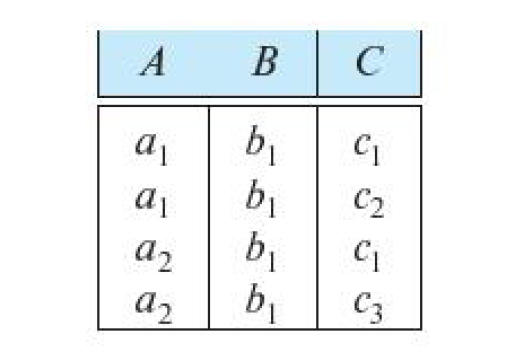
\includegraphics[width=5cm]{./images/7.2.png}
		\caption{7.2}
	\end{figure}
	
	
	\section*{7.2 解答}
	
	非平凡的函数依赖有:$ A \rightarrow B $和 $ C \rightarrow B, $以及它们逻辑上隐含的依赖:$ AC \rightarrow B$
	
	由于第一和第三个元组具有相同的 $ C $但不同的 $ A $值,所以他们直接不存在函数依赖。同理,其他的关系也不存在函数依赖
	
	故非平凡函数依赖有:$ A \rightarrow B $和 $ C \rightarrow B, $以及$ AC \rightarrow B$
	
	\section*{7.14} 
	Show that there can be more than one canonical cover for a given set of functional dependencies, using the following set of dependencies:
	$
	X \rightarrow YZ, \quad Y \rightarrow XZ, \quad Z \rightarrow XY.
	$
	
	\section*{7.14 解答}
	
	考虑第一个函数依赖。
	
	可以验证 $Z$ 是 $X \to YZ$ 中的冗余项并删除它。验证 $X$ 是 $Y \to XZ$ 中冗余并删除它。验证 $Y$ 是 $Z \to XY$ 中冗余并删除它。得到规范覆盖 $X \to Y, Y \to Z, Z \to X$。
	
	或者也可以验证 $Y$ 是 $X \to YZ$ 中冗余并删除它。验证 $Z$ 是 $Y \to XZ$ 中冗余并删除它。验证 $X$ 是 $Z \to XY$ 中冗余并删除它。得到规范覆盖 $X \to Z, Y \to X, Z \to Y$。
	
	\section*{7.15} 
	The algorithm to generate a canonical cover only removes one extraneous attribute at a time. Use the functional dependencies from Exercise 7.14 to show what can go wrong if two attributes inferred to be extraneous are deleted at once.
	
	\section*{7.15 解答}
	
	以删除 $X \to YZ$ 中的冗余项为例,如果一次性删除了 $Y$ 和 $Z$ 。删除这两个属性将导致无法再推断出 $X \to YZ$ 的函数依赖集。
	
	如果删除 $Y$ 会导致 $Z$ 不再是多余的,删除 $Z$ 会导致 $Y$ 不再是多余的。
	
	所以规范的覆盖算法一次只能删除一个元素,以避免上述情况
	
\end{document}
